\documentclass[11pt,a4paper]{article}
\usepackage{amsmath}
\usepackage{amsfonts}
\usepackage{amssymb}
\usepackage{graphicx}
\usepackage{hyperref} %inserting urls
\usepackage{nameref}
\usepackage{pdfpages}
\graphicspath{{Graphics/}} %Setting the graphicspath
\usepackage[utf8]{inputenc}
\usepackage[english]{babel}
\usepackage{lmodern}
% caption einr
\usepackage{caption}
\captionsetup{singlelinecheck=false,
	font=small,
	labelfont=bf,
	format=hang,
}
% Operators
\DeclareMathOperator*{\argmin}{argmin}
\DeclareMathOperator*{\argmax}{argmax}

% Appendix Chapters show in  TOC
% End Appendix Chapters show in  TOC

% Fakesubsection for Appendix
\newcommand{\fakesubsection}[1]{%
	\par\refstepcounter{subsection}% Increase subsection counter
	\subsectionmark{#1}% Add subsection mark (header)
	\addcontentsline{toc}{subsection}{\protect\numberline{\thesubsection}#1}% Add subsection to ToC
	% Add more content here, if needed.
}
% End Fakesubsection for Appendix

\author{Sebastian Knigge}
\begin{document}
	
\tableofcontents
	
\section{Introduction and Organization of the Thesis}
	
Even if the amount of data increases inexorably due to the permanent collection of online data, plus there are always new and better methods to derive good forecasts from big data, it is still difficult for algorithms to extract information from unstructured data. The amount of text data does not increase as quickly as the amount of structured user data. However, it should not be ignored that the written word still has an immensely high -if not the highest - information density for the human mind. Text is the primary and most accurate way to transfer and store complex information. In a nutshell: while machines and algorithms think in numbers, humans still think in words and text. A major challenge of machine learning will be to extract and link information from unstructured data such as text.\\
\ \\
One field of computer science is already addressing the topic of text data. This is Natural Language processing and Information Retrieval (see Chapter \ref{sec:NLP}). In the past, probabilistic approaches have been considered especially promising by researchers (see e.g. \cite{Manning1999}). However, the success of methods depends greatly upon the text data to which they are applied and on the desired output. It is therefore equally important to address the methods and models used, as well as to describe the use case in detail when conducting research in this area. Winter et al. for example characterized regulatory documents and guidelines via KNN \cite{Winter2017}. In this thesis, I would like to follow Winter's work thematically. I will examine related procedures and new, completely different methods and approaches to characterize regulatory documents.\footnote{When comparing the two works, however, note the difference in the topic of the documents analyzed.}\\
\ \\
In this work I adhere to the paradigms of Dejong's 1979 work in the field of natural language processing. He was the first researcher in this area to move away from the story-specific approach by testing the accuracy of his program to develop a more robust model \cite{DeJong1979}. I will even go a step further by optimizing my model with completely different data than that of what it will later be tested on. By doing so I try to reduce the overfitting of the model to the chosen topic and develop a universal tool for text classification. Specifically, I will train my approach for classifying text documents on a relatively large set of textbook chapters. I will optimize the models and their hyperparameters and test the optimized models with a smaller set of regulatory documents from EUROSTAT.\\
\ \\
In \textbf{Chapter \ref{sec:NLP}} I will discuss the evolution of natural language processing. The different approaches and methods will be summarized and the reader will be given a general overview of the context of this work.\\
\textbf{Chapter \ref{sec:Models}} presents the models used and the form of application is described in detail. The two methods used do not only differ in terms of their underlying models, but also their different tasks. Different methods of fitting and the implementation are covered.\\
In the following sections of this paper, two examples (respectively in \textbf{Chapter \ref{sec:analysis} and Chapter \ref{sec:example2}}) are presented. First, an introductory example with data from various textbooks is analyzed. In \ref{Example1} an LDA model is adapted to cluster the data. In \ref{sec:ANN.example} a neural network is built up piece by piece, in order to classifiy new books or chapters.\\
Based on the models in Chapter \ref{sec:analysis}, in \ref{Example2} another LDA model is developed to logically organize a collection of 28 regulatory documents and guidelines. In a second step (section \ref{Example2_ANN}), new documents are to be classified according to these groups.\\
To conclude, in \textbf{Chapter 6} the results of both examples are summarized and the importance of such a process of clustering and classification is outlined.\\
In order to give the reader a deeper insight into the examples and results and to ensure reproducibility, the \textbf{Appendix} contains four Documentation-pdfs in which the entire code and all results are presented in an edited form.


	
	

\section{Natural Language Processing and Information Retrieval} \label{sec:NLP}

The reason for the current relevance of the topic NLP is obvious. However	 what does the concept of natural language processing actually cover and into which research field is it to be classified? It is worth looking at how NLP has evolved over the years and where it originated in order to better understand what this area encompasses and what it does not. Since the origins of NLP lie in computer science, especially in Artificial Intelligence, NLP and AI share the same approaches. For a short review of the motivation of AI, see section \ref{ANN_development}.  \\
\ \\
“Between about 1960 and 1985, most of linguistics, psychology, artificial intelligence, and natural language processing was completely dominated by a \textbf{\textit{rationalist}} approach” \cite[p. 4]{Manning1999}. In other words, procedures for NLP were completely static, fix-programmed solutions for processing text data. Books like \cite{Noble1988} followed this approach until the late 80s. Whereby the enthusiasm gradually, just like for artificial intelligence itself, decreased and arose cyclical.\\
\ \\
The second school of thought mentioned by Manning and Schütz is the \textit{\textbf{empiristic}} approach.
This is based upon the assumption, that one “can learn the structure of language by specifying a general model and then learning the values of the parameters by applying statistical modeling and machine learning methods to large amount of observed language” \cite[p. 253]{Martinez2010}. What finally led to the breakthrough of NLP in its current form, is what Manning defines as statistical NLP. I.e. all quantitative approaches for automatization NLP, which includes probabilistic modeling, as well as information theory, and linear algebra. This thesis will focus on methods related to this approach.\\
Some of this work could even advance a step further. Deep learning (see \ref{ANN_development}) was indeed already invented in 1999 - at the time of the division of the definition Mannings in its basic outlines - but still received far less attention than today. One could therefore call NLP via deep learning a subcategory of the empirical approach in its own right, and possibly even list "deep NLP” alongside Statistical NLP.\\
\ \\
Statistical NLP always considers recurring patterns and structures in the context of certain texts and does not examine the whole language as such. This approach is no new invention by NLP researchers, but has been used by linguists even prior to computer science (see \cite{Harris1951}). A collection or body of texts is called a \textbf{\textit{corpus}}, which means "body" in Latin. In the course of this work we will also mention several corpora, which refers to multiple collections of texts.\\
\ \\
In this thesis so called topic models are studied and applied. David M. Blei defines topic models “as algorithms for discovering the main themes that pervade a large and otherwise unstructured collection of documents. Topic models can organize the collection according to the discovered themes”\cite{Blei2012}. This definition may therefore apply to both clustering and classification algorithms, even if many authors will refer to clustering algorithms in the context of topicmodels. You will find a brief introduction to clustering and classification models in the use case in Chapter \ref{sec:analysis}.\\
\ \\
Another important term in the research area of this thesis is information retrieval (IR). IR means to give access to a subset of documents of a corpus, which are relevant to a user’s query. This deals with computer-aided searches for complex contents and belongs to the fields of information science, computer science and computational linguistics. According to David Grossmann et al. IR refers to a search that might cover information of any kind, e.g. text data as well as video-, image-, sound data, or even DNA sequences. The field where LDA and IR overlap is document retrieval \cite{Grossmann2004}. Thus, most procedures we are discussing in this thesis might not solely fall into the topic NLP but also IR. By veering into this direction, it is intended for the reader to better understand the connection to this topic and at which intersection it is located. \\
\ \\
In addition, there is a further differentiation of methods concerning natural language processing. One can also distinguish text interpretation with regard to the tasks one intends to accomplish with it. \cite{Jacobs1993} distinguishes between three common tasks:
\begin{enumerate}
	\item \textit{Information Retrieval}: The task to find a subset of a corpus, which contains information concerning a user’s query.

	\item \textit{Data extraction}: The task to bring texts of a corpus of a particular domain into a pre-defined key structure, suitable for use in a traditional database.

	\item \textit{Text categorization}: Separating documents of a corpus into meaningful groups.
\end{enumerate}
The tasks dealt with in this paper may perhaps be best assigned to the last area. On the one hand, I specifically target the task text categorization by dividing a corpus of documents into a predefined number of groups. On the other hand, I try to assign new documents to these groups.\\
\ \\
In Chapter \ref{sec:NLP}, I will discuss the evolution of natural language processing. The different approaches and methods will be summarized and the reader will give a general overview regarding the context of this work.\\
Chapter \ref{sec:Models} presents the models used and describes the form of application in detail. The two methods used here do not only differ in terms of their underlying models, but also by their different tasks.












\section{Discussed Models} \label{sec:Models}

This section will discuss the two Topic modeling approaches which will be studied in this Thesis. The aim of both procedures is to assign one or more topics to different documents. Even if the vocabulary and the notation are similar for both approaches, the notation should be resumed at the beginning of the description of each model. The basic structural notation of the data consists of the following variables.

A collection of documents is called corpus $D=(\textbf{w}_1,\dots , \textbf{w}_M)$. It consists of $M$ documents $\textbf{w}=(w_1,\dots, w_N)$ which represents each of the $N$ words $w_i$ in the vocabulary. These words are vectors of length $V$. $V$ refers to the length of a vocabulary which holds all the words occurring in the corpus. The vector for a specific word $w_i$ contains all 0 except for index $j\in\{1,...,V\}$ which represents this very one word in the vocabulary. This specific system for storing the corpus is called \textbf{\textit{bag-of-words}} format.
This notation may be extended through the addition of indices for documents, but this is done neither here nor in the standard literature on topic models due to its unnecessary complexity.


% MODEL LDA Introduction
\subsection{LDA Model}\label{sec:LDA}

Latent Dirichlet Allocation is a Bayesian approach and is often associated with hierarchical models \cite{Gelman2014}. This idea is based on the representation of exchangeable random variable as mixtures of distributions as discussed by de Finetti.  Given that documents $\textbf{w}$ and words $w_i$ in each document - both considered as random variables in this setting - are exchangeable in such a way, a mixed model such as the LDA model is appropriate \cite{Blei2003}.

The following notation is used in conjunction with the LDA model. Let $z_j$ be the topics with $j\in\{1,\dots,k\}$. In the LDA setting we assume for  every topic $z_j$ there is a term distribution
$$\beta_j \sim Dir(\delta)$$
We further assume each document w has a distribution of topics.
$$\theta \sim Dir(\alpha)$$
Then each word $w_i$ of $\textbf{w}$ is generated by the following process:

\begin{enumerate}
	\item Choose $z_i \sim Mult(\theta)$
	
	\item Choose $w_i \sim Mult(\beta_i)$ This distribution will be referred to as $p(w_i|z_i,\beta)$
\end{enumerate}
\ \\
You can summarize this setup in a plate diagram as shown in figure \ref{fig:PlateDiagram}. The notation above, which is also used within the diagram, coincides with the notation of \cite{Hornik2011}.\\


\begin{figure}[h]
	\centering
	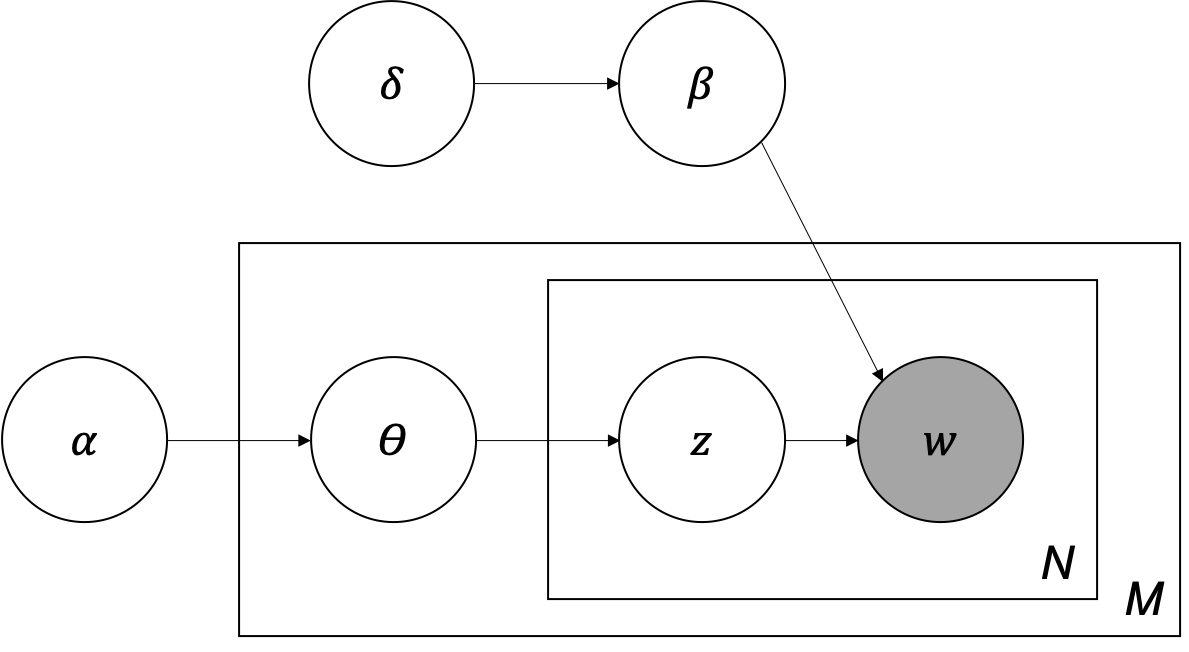
\includegraphics[width=0.5\textwidth]{LDA_Plate_Diagram.png}
	\caption{Well-established plate diagram for the standard LDA model extended by the parameter $\delta$. The slightly bigger box represents the generative model of the corporis $M$ documents. The smaller plate represents the iterative generation process of the $N$ words of each document with the aid of the topics. See also "smoothed LDA model" in \cite{Blei2003}  for comparisons.}
	\label{fig:PlateDiagram}
\end{figure}
\ \\
In order to estimate the model's parameters, the first step is to calculate posterior distribution, which can be done by dividing the joint distribution by the marginal distribution.

\begin{align}\label{posterior}
p(\theta,\textbf{z}|\textbf{w},\alpha,\beta)= \frac{p(\theta,\textbf{z},\textbf{w}|\alpha,\beta)}
{p(\textbf{w}|\alpha, \beta)}
\end{align}
The joint distribution numerator can be derived with the following calculation:

\begin{align}\label{joint}
p(\theta,\textbf{z},\textbf{w}|\alpha,\beta)=p(\theta|\alpha)\prod_{i=1}^{N}p(w_i|z_i,\beta)\ p(z_i|\theta)
\end{align}
One can obtain the marginal distribution of a document $\textbf{w}$, by integrating out the parameter $\theta$ and summing up the topics $z_j$. Nevertheless, this expression is intractable.
\begin{align}\label{marginal}
p(\textbf{w}|\alpha, \beta)=\int p(\theta|\alpha) \left( \prod_{i=1}^{N} \sum_{z_i}p(z_i|\theta)p(w_n|z_i,\beta) \right) d\theta
\end{align}
\ \\
The literature divides the approaches to calculating posterior distribution into two main categories.\cite{Blei2012} distinguishes between-sampling based algorithms and variational algorithms. \cite{Powieser2012} lists a total of 6 algorithms that can be used to estimate parameters in the LDA model. This thesis will be confined to the two most cited and most used members of the two main groups. One approach is to simulate the posterior density by iteratively sampling - the so-called Gibbs Sampling method. The second approach is a deterministic method, a modified version of the well-known EM algorithm \cite{Dempster1977}: the Variational EM algorithm (VEM algorithm) \cite{Wainwright2008}. In the following two sections the both approaches are roughly outlined to give the reader some insight into the Bayesian inference underlying the algorithms.

\subsubsection{Variational EM Algorithm}

In the VEM algorithm for the LDA model is a mean field approach which varies the steps E and M of the EM algorithm in a way such that this algorithm becomes solvable. Note that the main problem in calculating marginal distribution lies in deriving the conditional probability of hidden variables in the observed values ('evidence'). Variation in the EM algorithms arises mainly from approximating the directly intractable E step.  Rewriting the log of the border density of $\textbf{w}$ as follows in (\ref{marginal2}), results in a downward estimation of marginal density given Jensen's inequality.
\begin{align}\label{marginal2}
\log p(\textbf{w}|\alpha, \beta) &= \log \int \sum_{z} 
p(\theta,\textbf{z},\textbf{w}|\alpha,\beta)d\theta\\
& =\log \int \sum_{z} \frac{p(\theta,\textbf{z},\textbf{w}|\alpha,\beta) q(\theta,\textbf{z})}{q(\theta,\textbf{z})}d\theta\\
&\geq \int \sum_{z} q(\theta,\textbf{z})\log p(\theta,\textbf{z},\textbf{w}|\alpha,\beta) d\theta - 
\int \sum_{z} q(\theta,\textbf{z})\log q(\theta,\textbf{z})d\theta\\
&= \mathbb{E}_q[\log p(\theta,\textbf{z},\textbf{w}|\alpha,\beta) ]-
\mathbb{E}_q[\log q(\theta,\textbf{z})] \label{KL}
\end{align}
Here $q(\theta,\textbf{z})$ is an arbitrary distribution which can be called the variational distribution. 
\begin{align}
q(\theta,\textbf{z})\widehat{=}q(\theta,\textbf{z}|\gamma,\phi)
=q(\theta|\gamma) \prod_{i=1}^N q(z_i|\phi_i)
\end{align}
The right hand side $L(\gamma,\phi,\alpha, \beta):=\mathbb{E}_q[\log p(\theta,\textbf{z},\textbf{w}|\alpha,\beta) ]-
\mathbb{E}_q[\log q(\theta,\textbf{z})]$ is referred to as the 'lower bound'. It can be shown that $\log p(\textbf{w}|\alpha, \beta) - L(\gamma,\phi,\alpha, \beta)$ is the Kullbak Leibler divergence ($D_{KL}$) of the true posterior and the variational distribution. From equations (\ref{marginal2})-(\ref{KL}) follows that:
\begin{align}\label{equality}
\log p(\textbf{w}|\alpha, \beta)= D_{KL}(q(\theta,\textbf{z}|\gamma,\phi)||p(\theta,\textbf{z},\textbf{w}|\alpha,\beta)) + L(\gamma,\phi,\alpha, \beta)
\end{align}
Since the marginal distribution is fixed, we conclude that minimizing the KL-divergence is equivalent to maximizing the lower bound (see \cite{Jordan1999} and \cite{Wainwright2008}, for details of the derivation of the lower bound see \cite{Blei2003}).
\begin{align}
(\gamma^*, \phi^*) &= \argmin_{\gamma, \phi}D_{KL}(q(\theta,\textbf{z}|\gamma,\phi)||p(\theta,\textbf{z},\textbf{w}|\alpha,\beta))\\
&= \argmax_{\gamma, \phi} L(\gamma,\phi,\alpha, \beta)
\end{align}\\
\\
The EM algorithm thus is to use the variational distribution $q(\theta,\textbf{z}|\gamma^*(\textbf{w}), \phi^*(\textbf{w}))$ instead the posterior distribution $p(\theta,\textbf{z},\textbf{w}|\alpha,\beta)$. Now the two steps of the VEM algorithm are:
\begin{itemize}
	\item [(1)]\textbf{E step} Optimize the variational parameters $\theta$ and $\phi$ for every document in the corpus. This can be done analytically by deriving the derivatives of the KL divergence. And set them to zero.
	\item [(2)] \textbf{M Step} Maximize the lower bound using the optimized parameter of the E step with respect to $\alpha$ and $\beta$.
\end{itemize}


\subsubsection{Gibbs Sampling}

The second method to approximate the posterior distribution is Gibbs sampling, a form of the Monte Carlo method. Instead of calculating the distributions for $\beta$ and $\theta$, the primary task is to find the posterior distribution over $\textbf{z}$ given the document $\textbf{w}$. Gibbs sampling is also known as a Markov Chain Monte Carlo method. The name refers to the simulation process by which a chain of values is simulated whose limiting distribution desirably converges against the true distribution \cite{Griffiths2006}. (\ref{Gibbs}) shows the distribution, which is sampled from iteratively.
\begin{align}\label{Gibbs}
p(z_i=j|z_{-i},w)\propto \frac{n_{-i,j}^{(l)}+\delta}{\sum_t n_{-i,j}^{(t)}+V\delta}
\frac{n_{-i,j}^{(d_i)+\alpha}}{n_{-i}^{(d_i)}+k\alpha}
\end{align}
\makebox[1cm][l]{$z_{i}=j$} 		... \makebox[5cm][l]{word-topic assignment of word $i$ to topic $j$}\\
\makebox[1cm][l]{$z_{-i}$}   		... \makebox[4cm][l]{vector of word-topic assignments without the entry for word $i$}\\
\makebox[1cm][l]{$n_{-i,j}^{(l)}$}	... \makebox[4cm][l]{number of times the $l$th word in the vocabulary is assigned to }\\
\makebox[1cm][l]{}						\makebox[4cm][l]{\ \ \ \ topic $j$, not including the assignment for word $i$}\\
\makebox[1cm][l]{$d_i$}				... \makebox[4cm][l]{document in the corpus which includes word $i$}\\
\makebox[1cm][l]{$\delta,\alpha$} 	... \makebox[4cm][l]{parameters of the prior distributions for $\beta$ and $\theta$}\\
\\
The word-topic distributions $\beta_{j}^{(l)}$ for the words $l=1,...,V$ and topics $j=1,..,k$ and topic-document distributions $\theta_j^{(d)}$ for the documents $d=1,...,D$ and the topics $j=1,...,k$ will be of particular interest. (\ref{Gibbs:beta}) and (\ref{Gibbs:theta}) shows the predictive distributions denoted as "estimators". 
\begin{align}
\hat\beta_{j}^{(l)}&=\frac{n_{-i,j}^{(l)}+\delta}{\sum_t n_{-i,j}^{(t)}+V\delta} \label{Gibbs:beta} \\
\hat\theta_j^{(d)}&= \frac{n_{-i,j}^{(d_i)+\alpha}}{n_{-i}^{(d_i)}+k\alpha} \label{Gibbs:theta}
\end{align}
For derivation and more details regarding the Gibbs sampling procedure see \cite{Griffiths2006}.

\subsubsection{Implementation}

In this thesis, the implementation of the LDA model and its estimation is mainly based on using the package \texttt{topicmodels} of Kurt Hornik. The package \texttt{topicmodels} can apply both the VEM algorithm as well as Gibbs sampling in order to fit the model. In addition, the package \texttt{tidytext} is used for text structuring and embedding. Whereby there are other packages besides this implementation of the LDA model, \texttt{topicmodels} is particularly convenient, because \texttt{tidytext} was designed by its developers to work perfectly in combination with \texttt{topicmodels} \cite[p. 89]{Silge2017}.


\subsection{Artifical Neural Networks}

Artificial neural networks (ANN) are much more versatile than the LDA model. There are not only various forms of artificial neural networks, but also a very large number of application areas. Much like machine learning procedures in general, also deep learning algorithms are divided into two broad categories: supervised learning, where a superset instance provides the algorithm with the output required to learn, and unsupervised procedures that internally train predefined models to find patterns in the input signals. In this chapter we will focus heavily on the former group of ANNs. Also, this chapter is intended to give the reader an overview of the research on neural networks as well as the background of their development. \\
\subsubsection{Development} \label{ANN_development}
Research on ANNs dates back to the 1940s, when \cite{McCulloch1943} introduced the so called “M-P neuron”. Whereby this neuron had only a bivariate input and output, Rosenblatt later extended this idea to a network of M-P neurons, which allowed to set up a simple classification algorithm \cite{Rb1958}. A perceptron in its basic form (single perceptron) is a binary classifier. \\
\\
Imagine input data of a simple perceptron in the form of a matrix. 
$$X= \left[
\begin{array}{rrr}                                
x_{11} & \dots & x_{1k} \\                                               
\vdots & \ddots & \vdots \\                                               
x_{n1} & \dots & x_{nn} \\                                             
\end{array}
\right] = \left[
\begin{array}{r}                                
\textbf{x}_{1} \\                                               
\vdots \\                                               
\textbf{x}_{n} \\                                             
\end{array}
\right]
$$ 
The dependent variable thus is a vector $\textbf{y}=y_1,…,y_n$, with $y_i\in \{0,1\}$. Consider the lines of the X mtrix as vectors $\textbf{x}_1,…,\textbf{x}_n$, with $\textbf{x}_i\in\mathbb{R}^k$. The entries of each of the vectors are weighted with $\textbf{w}=w_1,\dots,w_k$ with $w_j \in \mathbb{R}$ and aggregated in a function $h$ e.g. a sum.
$$h(\textbf{x},\textbf{w})=\sum_{j=1}^kx_jw_j$$
Using a so called "activation function" $h$ is mapped to the output space, which is in this case $O=\{0,1\}$. At this point a step function serves as activation function.
$$a \circ h(\textbf{x},\textbf{w}) = \begin{cases} 0 \text{ if } h(\textbf{x},\textbf{w}) \leq 0 \\ 1 \text{ else}\end{cases}$$
The matrix $X$ is passed vector by vector to the percepron and the output is compared with the values for $\textbf{y}$. During this procedure the weights are iteratively tuned by a simple updating algorithm using the pairs $\textbf{x}_i$ and $y_i.$

\begin{figure}[h]
	\centering
	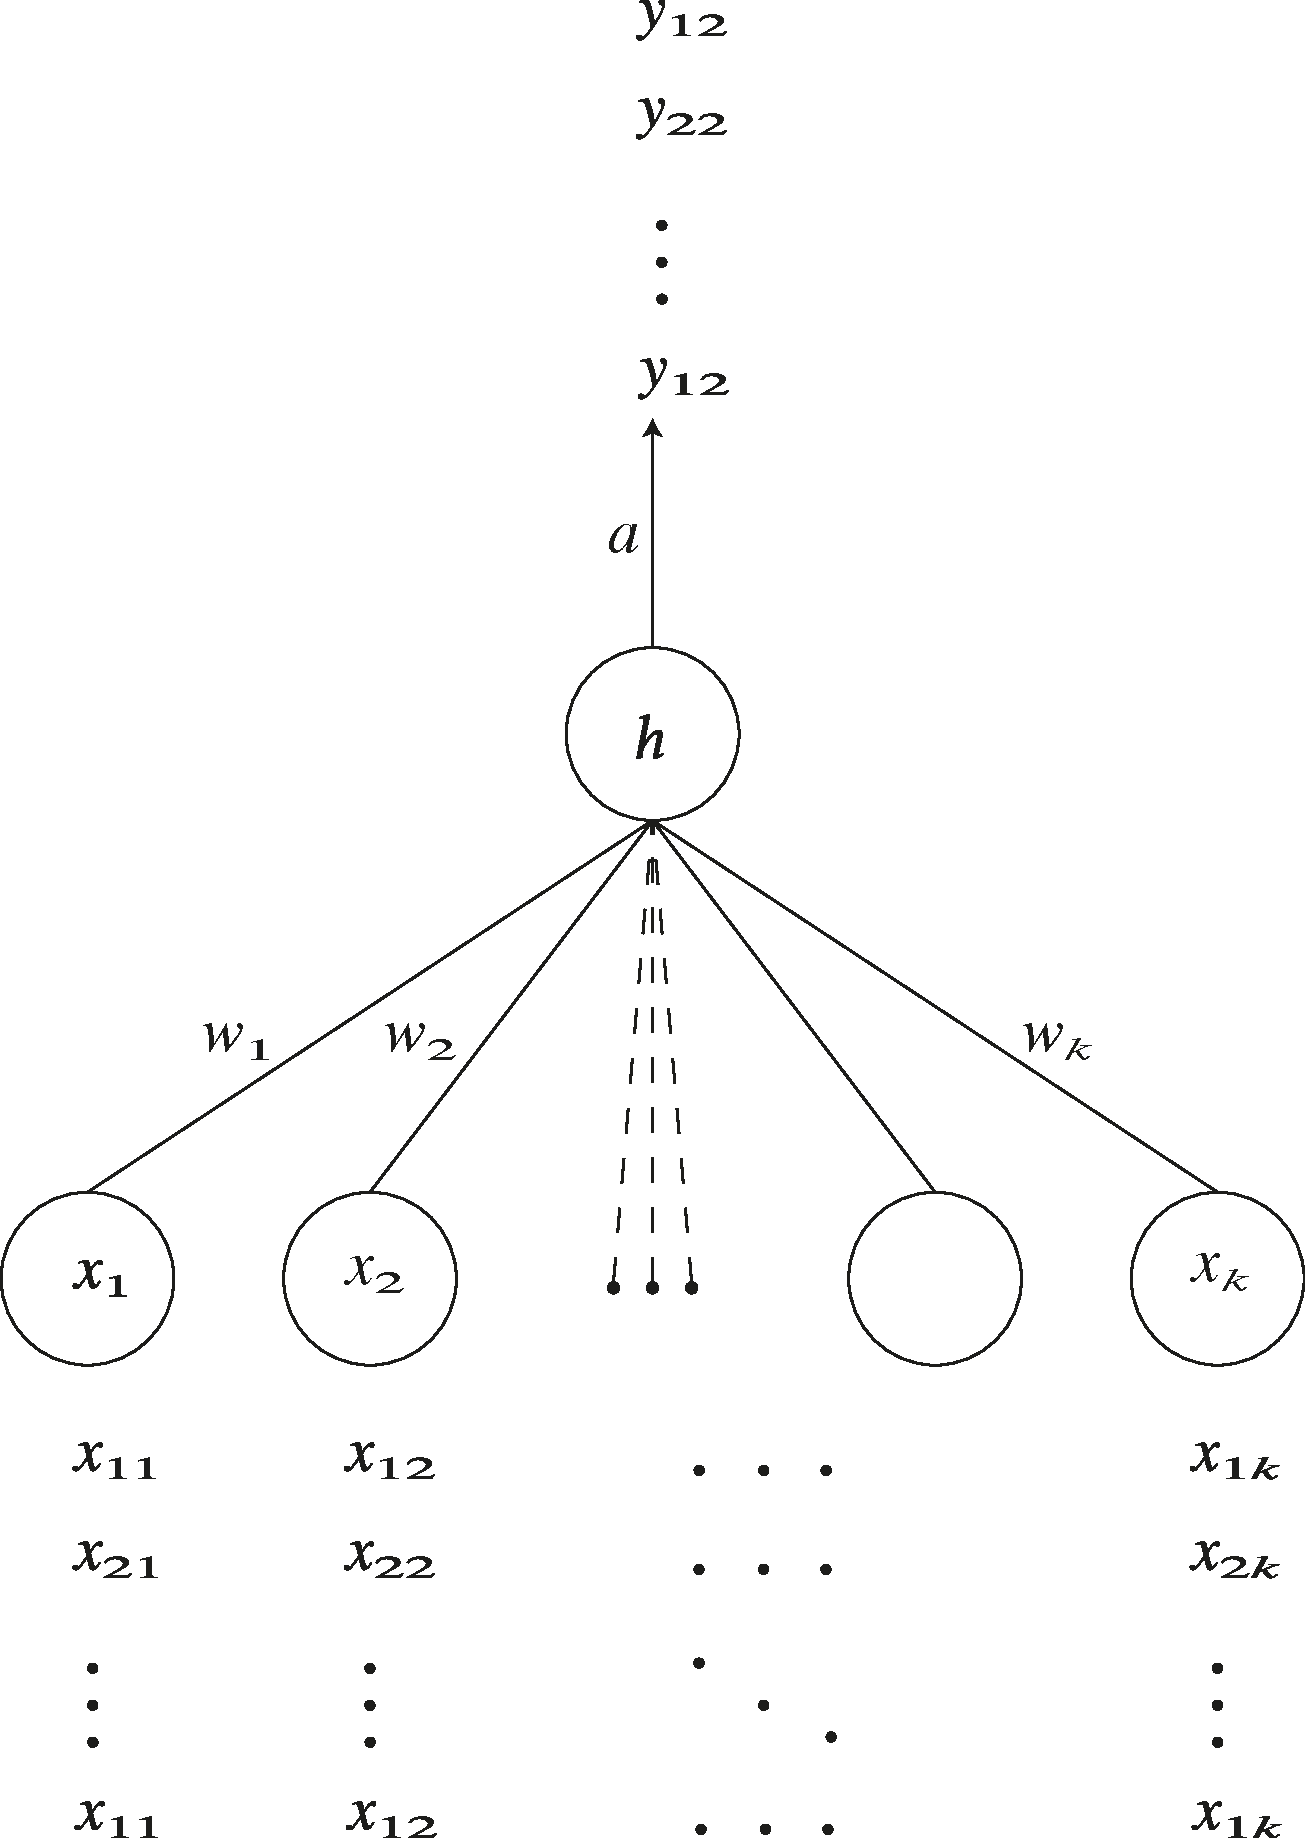
\includegraphics[scale=0.4]{simple_perceptron.pdf}
	\caption{Schematic diagram of a simple perceptron by \cite{Rb1958}}
	\label{simple_perceptron}
\end{figure}
\ \\
The algorithm of the simple perceptron is schematically shown in Figure \ref{simple_perceptron}. This diagram corresponds to the common representation in education \cite{Mekherjee2019}, although a horizontal perspective is often chosen.\\
\\
If this basic perceptron is used in a clever way, designs can be developed that have many different application possibilities. For example, a sigmoid function can be used as an activation function instead of the step function. So the output layer will not project into the $\{0,1\}$ space, but into a probability space. If you add several nodes with the sigmoid activation function rather than a single output, you basically obtain the architecture that is also called multivariate logistic regression \cite{Bahjat2006}. In that case the model can be estimated by an individual calculation of logistic regressions for each node in the output layer. This allows to classify not only two classes, but an arbitrary number (see the network architecture of Figure \ref{adaption_perceptron}). \footnote{Note that in this setting the dependent variable must be one-hot encoded.}\\
\begin{figure}[h]
	\centering
	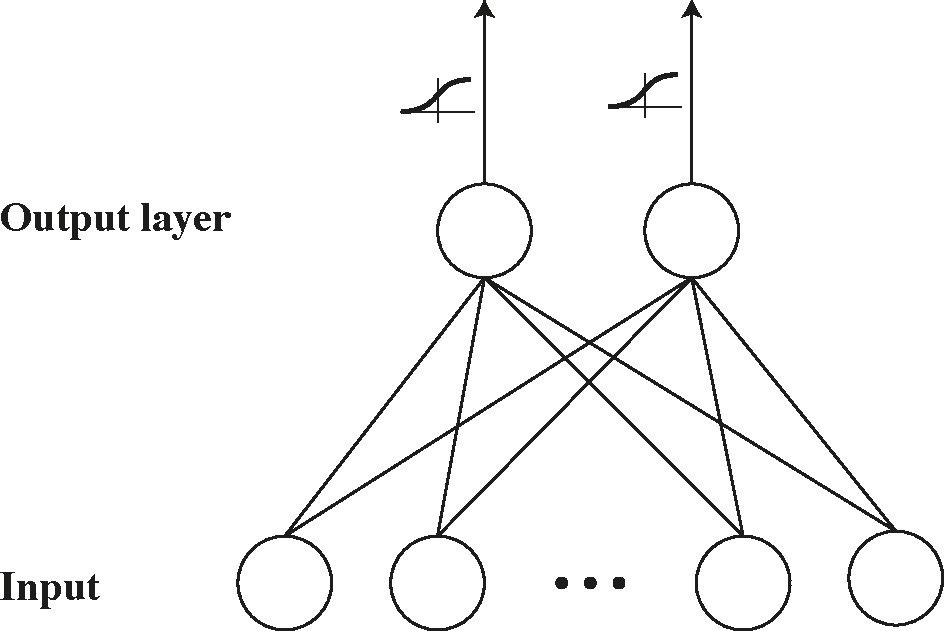
\includegraphics[scale=0.5]{adaption_perceptron2.pdf}
	\caption{Schematic diagram of an adapted Rosenblatt-perceptron network}
	\label{adaption_perceptron}
\end{figure}
\ \\
Shortly following the publication of these results, which would lay the foundation for later neural networks, ANN research had to suffer a severe setback after Minsky and Papert \cite{Minsky1969} were able to prove that perceptrons cannot provide a suitable solution in certain basic scenarios. It is possible to separate two clusters by a hyperplane with the perceptron. However, if the two groups could not be separated completely, the perceptron fails. For instance, it was impossible to find a solution for data generated with an \textit{x-or} function (also called "exclusive or" function).\\
\ \\
Although the researchers Minsky and Papert showed that the perceptron in this form cannot solve the “xor problem”, they argued that extending the simple perceptron to a multi layer perceptron solves this problem, if it was feasible to train this model. Instead of just one input layer and one output layer, an MLP may include an arbitrary number of hidden layers in between. Figure \ref{figure:MLP} shows the structure of such an network. However, training a model using Rosenblatt's naive optimization algorithm of the perceptron would not have been feasible.\\
\begin{figure}[h]
	\centering
	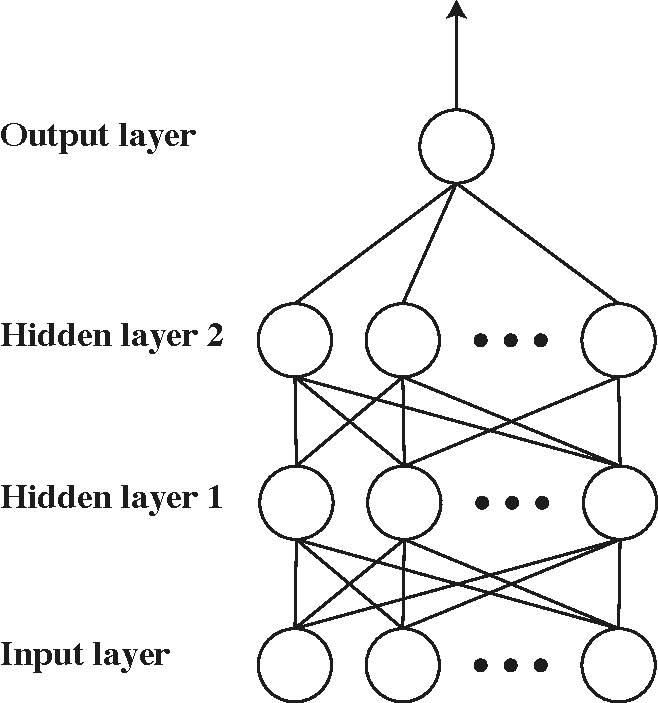
\includegraphics[scale=0.6]{MLP.pdf}
	\caption{Schematic diagram of an multi layer perceptron (MLP)}
	\label{figure:MLP}
\end{figure}
\ \\
\subsubsection{Backpropagation}
The procedure used to optimize the weights of a multilayer perceptron is called backpropagation. This method was first applied to neural networks by Webos - as part of his dissertation \cite{Werbos1974}- and still works the same way to this day. It is important to use a sigmoid function instead of the step function which is used in the perceptron, as this function is differentiable.  Assume a random initial distribution of the weights $w_1,\dots,w_d$ for a network with $d$ layers, which are the starting values for the update procedure. Let $\tau_i$ be the number of units in layer $i$. So layer $i$ can be denoted as function $f_{w_i}$ and the whole network as a chain of functions.
\begin{align}\label{network_chain}
	\hat{y_i}=f_{w_d}(f_{w_{d-1}}(...(f_{w_1}(x_i))))=f_{w_d}\circ f_{w_{d-1}} \circ \dots \circ f_{w_1}(x_i)
\end{align}
The goal is to update the weights of each layer in sucha way as to minimise a selected loss function $L(w_1,\dots,w_d)$. A common loss function is for example quadratic loss: $L=\frac{1}{2}\sum_{i=1}^n(\hat{y_i}-y_i)^2$\\
The backpropagation algorithm consist of the 3 following roughly outlined steps.
\begin{enumerate}
	\item \textbf{forward pass:} Calculation of the result $y_i$ for all units at the set weights
	\item \textbf{backward-sweep:} Each layer's derivatives are now calculated using the chain rule, step by step - starting with the output layer. For the output layer this is:
	\[\frac{\partial L}{\partial w_d}=\frac{\partial L}{\partial f_d(x_i)}\frac{\partial f_d(x_i)}{\partial w_d}	\]
	\item \textbf{updating:} Update the weights by an arbitrary optimization algorithm. E.g. steepest descent:
	$\Delta w_d=\alpha \frac{\partial L}{\partial w_d}$
	,where $\alpha$ is the learning rate
\end{enumerate}
Thanks to current software, the derivatives no longer have to be calculated for each node by hand, but the standard packages are capable of "symbolic differentiation" for certain network structures, which makes training neural networks comfortable \cite[p. 47]{Chollet2018}.\\
\ \\
Note: While Rosenblatt for the perceptron was actually inspired by the biological structure of the neurons in the brain, more complex “networks used by engineers are only loosely based upon biology”\cite{Hecht-Nielsen1988}.

\subsubsection{Implementation}
This thesis uses the \texttt{Keras R} package to create neural networks, a deep learning API (Application-Programming-Interfac) to deep learning backend engines, designed for \texttt{R} by Allaire in 2017. Keras is a so called “model-level” library, designed to set up complex neural net architectures using well arranged, high-level building blocks. As backend-engine the users are provided with TensorFlow, Theano and Microsoft Cognitive Toolkit. Using these backend engines computation may be processed seamlessly via CPU or GPU \cite{Chollet2018}.

% ANALYSIS OF TEXTBOOK CHAPTERS
\section{Analysis of Gutenberg Data}\label{sec:analysis}

In this first example, the chapters of individual books are classified, all of which sourced from the freely distributed Project Gutenberg. Project Gutenberg is a provider of over 60,000 free electronic books with the primary aim to “encourage the creation and distribution of eBooks”\cite{ProjectGutenberg}. The package \texttt{gutenbergr} \cite{gutenbergr} preprocesses the ebooks text data and downloads it. This convenient package in combination with the free repository allows the analysis of a large number of large text documents with a secure source and a big amount of meta information. For this analysis interesting information is e.g. Gutenberg id as key variable for fast identification of books, title, author and more importantly the categorization of project Gutenberg, the so-called Gutenberg bookshelf. Table \ref{titles:5books} lists all this information for a random sample of books downloaded from the Project Gutenberg.

\begin{table}[!htbp] \centering 
	\caption{Example book corpus} 
	\label{titles:5books} 
	\tiny
	\begin{tabular}{@{\extracolsep{2pt}} c|c|c|c} 
		\hline 
		\hline \\[-1.8ex] 
		gutenb. id & title & author & gutenberg bookshelf \\ 
		\hline \\[-1.8ex] 
		$2095$ & Clotelle: A Tale of the Southern States & Brown, William & African American Writers \\ 
		$6315$ & The Awakening of Helena Richie & Deland, Margaret & Bestsellers, American\\ 
		$6971$ & Judaism & Abrahams, Israel & Judaism \\ 
		$7635$ & The Disowned — Volume 05 & Lytton, Edward and Baron & Historical Fiction \\ 
		$10319$ & Dave Darrin's Third Year at Annapolis & Hancock, Harrie Irving & Children's Book Series \\
		\hline 
	\end{tabular} 
\end{table} 
\ \\
In order to test NLP models, two questions can be examined on the basis of these simple text documents. 
\textbf{Firstly (Q1), does a LDA cluster text documents similar to a human-driven classification?} In this case, this could be validated by the categorization into Gutenberg bookshelves. \textbf{And secondly (Q2), what is the best approach to reproduce such a classification using an ANN as a classification model?} \\
Since very large amounts of data have to be processed and analyzed in order to model the bookshelf classification for a big collection of books, a somewhat reduced approach will be used here. One breaks down a collection of books of different categories into chapters in order to cluster respectively classify these chapters as independent documents. Similarly, you could give an example, assuming $N$ books and separate their chapters and shuffle them, is it possible to use models to reassemble the chapters into stacks that can be assigned to individual books?\\
\ \\
The raw text record is now transformed into the tidy format of tidytext (i.e. one word per row). Now it is possible to remove unnecessary stop-words. These words are predefined and can be modified for the appropriate use case if necessary. The words stem from 3 sources, "onix", "SMART" and "snowball", whereas the latter two are pulled from the \texttt{tm} package \cite{tidytext}.  And the Onix stop words are taken from the publicly accessible site lextec.com. An example of stop words can be found in Table \ref{stopwords}.
\begin{table}[!htbp] \centering 
	\footnotesize
	\caption{Example of stop words from tidytext package} 
	\label{stopwords} 
	\begin{tabular}{@{\extracolsep{5pt}} cc} 
		\\[-1.8ex]\hline 
		\hline \\[-1.8ex] 
		word & lexicon \\ 
		\hline \\[-1.8ex] 
		many & SMART \\ 
		mrs & onix \\ 
		was & snowball \\ 
		sure & onix \\ 
		you're & snowball \\ 
		go & onix \\ 
		c & SMART \\  
		where & snowball \\ 
		then & SMART \\ 
		\hline \\[-1.8ex] 
	\end{tabular} 
\end{table} 
\\
Both models that are studied in this thesis, use a bag-of-words data set as input data. This means a matrix with the documents in the $M$ lines and the frequencies of the $V$ used words in the entries of the columns. The dimension - i.e. the number of words in this "dictionary" $V$ - may be reduced for two reasons. For one thing, a dimension reduction can reduce the fitting time of the model, for another thing, the diversity of the documents can be increased by skilfully reducing certain words, which occur equally frequently in all documents. Now this requires a special measure on which we decide which words to exclude. One can call this reduction of the bag-of-words dimensionality "embedding". In the course of this work 3 different embedding methods were tested. 
\begin{enumerate}
	 \item The reduction by the words that occur with a low frequency. 
	\item No dimension reduction, i.e. use of the full dictionary of all occurring words. 
	\item The reduction with the aid of the measure \textit{tf-idf}.
\end{enumerate}

\textit{tf-idf} is a combination of the term frequency and the inverse document frequency, defined as follows.
$$\text{\textit{tf-idf}}(t,d):=tf(t,d)\times idf(t)$$
$$tf(t,d):=\frac{f_{t,d}}{\sum_{t_i=1}^V f_{t_i,d}}$$
$$idf(t):=\ln\left(\frac{M}{n_{d'\in t}}\right)$$
\\
\makebox[1cm][l]{$t$} 		... \makebox[5cm][l]{term (word)}\\
\makebox[1cm][l]{$d$}   	... \makebox[4cm][l]{document}\\
\makebox[1cm][l]{$f_{t,d}$} ... \makebox[4cm][l]{frequency of term $t$ in document $d$}\\
\makebox[1cm][l]{$M$} 		... \makebox[5cm][l]{number of documents}\\
\makebox[1cm][l]{$n_{d'\in t}$}   	... \makebox[4cm][l]{number of documents containing term $t$}

\ \\
Even if “its theoretical foundations are considered less than firm by information theory experts”, \textit{tf-idf} “has proved useful in text mining” \cite{Silge2017}. In this thesis the term frequency and the \textit{tf-idf} are not to be used directly for the analysis of the texts but mainly for setting up the bag-of-words datasets. It shall be investigated whether the use of different embeddings has an influence on the text analysis itself.

% SUBSECTION
% Lda applied on Gutenberg Data
\subsection{LDA applied to Textbook Chapters} \label{Example1}

As LDA is a classification algorithm, the research question Q1 should be addressed first. I.e. to what extent does the clustering of the LDA model correspond to the mapping of chapters to books? In the first attempt only 6 books are sampled. That is, there are 6 categories, because as mentioned in \ref{sec:analysis} all these 6 books were taken from different bookshelves.\\
\ \\
As described in Chapter \ref{sec:LDA}, it is possible to calculate the LDA model by means of two different algorithms. These are the VEM algorithm and Gibbs sampling. In this study we examined both methods. Clearly, the algorithms may differ in the speed of the calculation. However, it does not have to be the case that both calculation methods deliver the same results.\\
\ \\
Three fundamentally different approaches should be distinguished for embedding:
\begin{enumerate}
	\item the entire dictionary, i.e. all words occurring in the corpus are used for the bag-of-words.	
	\item for the bag-of-words only words are used which occur at least 2 times in the whole corpus. This reduces the number of used words and therefore the dimension of the data by nearly 50\%.
	\item the bag-of-words is reduced by 50\% according to \textit{tf-idf}.
\end{enumerate}
These approaches are reviewed with regard to the goodness of the fit and the speed of the computation. One intuitively may assume that the calculation takes longer for data with higher dimensionality.\\
\ \\
For a clustering model there are two useful methods to evaluate the fit. On the one hand it is possible to fit the model with training data and to evaluate the goodness of the fit using the test data. On the other hand, it is a comparison of the classification of the model with the categories given by the data, whereby the model does not learn from these categories. The latter evaluation method is clearly less computationally intensive, and the comparison of the entire data set instead of only the test part of the data has a positive effect on the variance. Starting this analysis the second approach is used primarily.\\
\ \\
The findings of this study relating to the LDA model are documented in detail. You will find the documentation regarding the LDA model as well as the other models in the appendix. For the sake of clarity, a separate document with the corresponding results was created for each analyzed example and each model respectively. To ensure reproducibility, the entire code is attached to the work by means of these documentations, and will be published on GitHub as well.\footnote{\url{https://github.com/SebastianKnigge/Master_Thesis/tree/master/Documentations} }\\
\ \\
The computation of the LDA model via VEM takes a somewhat longer time in the two samples evaluated. In all cases investigated, i.e. across the two samples taken and for both VEM and Gibbs sampling, the calculation for the \textit{tf-idf} embedding appeared to be the fastest. The calculation time for embedding according to term frequency and full embedding differs less and the calculation of the term frequency embedding is not faster in every case. While a reduction via term frequency only cuts the most rarely used words, a reduction via \textit{tf-idf} also cuts out frequent words as long as they occur frequently in all documents. Thus, \textit{tf-idf} reduction has more impact on the distribution within each document compared to the effect of the term frequency reduction, which only affects the tails of the marginal distribution. This supports the assumption that a higher degree of difference in the documents has a positive effect on the calculation speed. Firgure \ref{fitting_time_tfidf} visualizes how the fitting time changes when reducing the bag-of-words to an arbitrary size via \textit{tf-idf}.\\
\begin{figure}[h]
	\centering
	\includegraphics[page=15, trim=70 400 0 0,clip,width=1.1\textwidth]{LDA_Documentation.pdf}
	\caption{Fitting time of Example 1 (6 Books) depending on the reduction of the bag-of-words. A big number of fraction stands for a bigger bag-of-words, i.e. less reduction. The blue smoothed curve is a Loess kernel. The drop in fitting time for the last few values of fraction might result from parallelization reasons.}
	\label{fitting_time_tfidf}
\end{figure}
\ \\
With regard to the quality of the fit, it is apparent that Gibbs sampling performs much better than models fitted by VEM. The best fit using VEM still shows a higher misclassification rate than the poorest fit using Gibbs sampling in the examples examined. It is reasonable to focus on Gibbs sampling in further analyses. For this reason we will only consider Gibbs sampling in Chapter \ref{Example2}.\\
\ \\
Surprisingly, the models with the \textit{tf-idf} embedding do not perform significantly better than the other approaches, as one might expect that more differentiated word distributions of documents not only allow a faster calculation, but also result in a higher accuracy. In fact, frequency 2 embedding provides better accuracy results throughout the studied examples.\\
It may be interesting to test embedding via \textit{tf-idf} for different values of reduction. So far, a reduction of 50\% has always been considered. In this case we measure $\textit{fraction}=1-\textit{reduction}$ (i.e. what fraction of the original bag-of-word remains after \textit{tf-idf} embedding). Figure \ref{misc.rate_tfidf} shows the misclassification rate for different values of fraction. We can obtain a general negative trend of the misclassification rate, for bigger values of fraction. This means the accuracy of the model increases with a larger bag-of-words, for the reduction via \textit{tf-idf}. However, there are also values of fraction where the accuracy for both examples improves compared to full embedding (i.e. fraction 1). However, this may also be overfitting of the parameter fraction, if for other samples for this value of fraction the accuracy is worse. This parameter needs to be optimized very carefully, taking into account the underlying documents and the application. In summary, \textit{tf-idf} embedding can achieve very good results if the fraction parameter is tuned. For a generic approach, however, this method is too vulnerable to over-fit and it is recommended to choose a reduction to term frequency $2$ as embedding method, if there is no further information about the data set.\\
\begin{figure}[h]
	\centering
	\includegraphics[page=14, trim=73 405 60 70,clip,width=0.55\textwidth]{LDA_Documentation.pdf}\includegraphics[page=16, trim=85 275 50 200,clip,width=0.55\textwidth]{LDA_Documentation.pdf}
	\caption{Misclassification rate depending on the reduction of the bag-of-words. A big number of fraction stands for a bigger bag-of-words, i.e. less reduction. The blue and red smoothed curves are a Loess kernels.}
	\label{misc.rate_tfidf}
\end{figure}
\ \\
It was also analyzed how the accuracy will change when using more categories. For this purpose the number of books was increased to 10. The fit via VEM was still much worse than the fit via Gibbs sampling. The model fitted with VEM showed a missclassification rate almost twice as high as the one fitted with Gibbs sampling. For both methods the accuracy deteriorated for more topics used. This sounds intuitive since the clustering algorithm now has to distinguish between more topics. The box plot in Figure \ref{fig:comparison_boxplot} illustrates the LDA algorithm in the different use cases. Here we are comparing the investigated cases. Clearly the difference in the misclassification rate between the examples with 10 and 6 categories becomes apparent. It also illustrates how different the two calculation methods - Gibbs sampling and VEM - are.

\begin{figure}[h]
	\centering
	\includegraphics[page=22, trim=70 400 0 0,clip,width=1.2\textwidth]{LDA_Documentation.pdf}
	\caption{Boxplot of the all examples analyzed. Split for the number of categories (books) as well as for the calculation procedures (VEM algorithm and Gibbs sampling).}
	\label{fig:comparison_boxplot}
\end{figure}
\ \\
Considering the second approach for evaluation mentioned in the beginning of this section, results regarding this procedure should be discussed as well. The classical method to evaluate the model is to split the data set into a training set and a test set, in order to fit the model on the training data and to evaluate it on the test data. To calculate valid results 59 random clustered samples were used with splits of 90\% training sample and 10\% test sample applied. The results for those models that were only fitted to a subset of the data are significantly worse than the comparable models that were trained and tested on the entire dataset. However, since here a clustering model is discussed that does not rely on training data, such as a classification model, it is technical correct to evaluate the model using training data.\\
But what do these results mean for the LDA model? Since this method aims at evaluating the fit on the basis of classifying new documents, it is basically an evaluation method for classification problems. It follows that the LDA model is a poor classification model for the use case analyzed. For this reason, I use another model to classify new documents, which is a neural network (see following section).

\subsection{ANN applied to Textbook Chapters} \label{sec:ANN.example}

In what context is it now possible to apply an artificial neural network to this data? Obviously neural networks are a very versatile tool, but here we focus on the reproduction of a known classification of the documents (chapters) by a suitable model. With the help of such networks in the sense of a classification algorithm, research question 2 will be addressed in this section. Again, for the shake of reproducibility the entire code including outputs of the computations can be found in the documentation in the appendix.\\
\ \\
Primarily the question shall be addressed whether a neural network is suitable as a classification algorithm for NLP with bag-of-words data. First of all, the architecture of the network used will be explained (see Figure \ref{fig:network_structure} for comparison).
\begin{figure}[h]
	\centering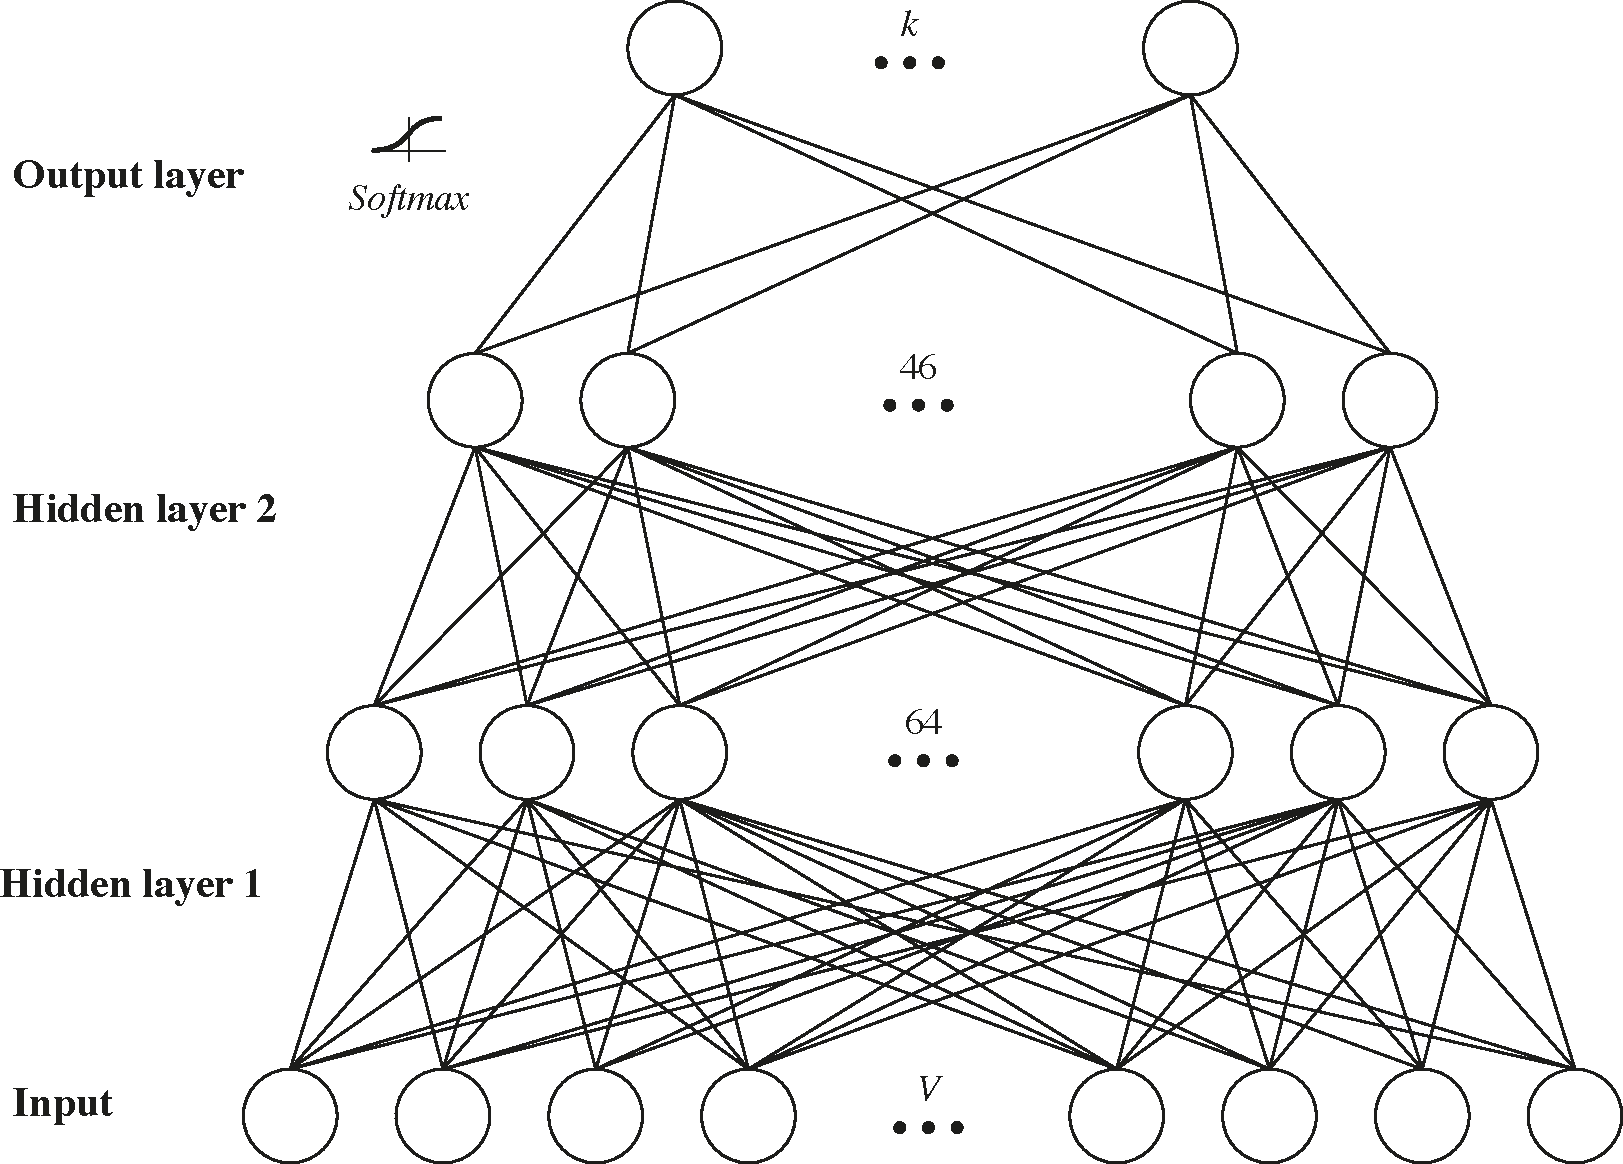
\includegraphics[width=1\textwidth]{network_structure.pdf}
	\caption{The network contains 3 layers. The input data is the the bag-of-words, which has dimension $V$. The first two layers are hidden, containing 64 and 46 neurons respectively. The last layer leads to the $k$ classes (here the number of topics or books). The activation function is softmax.}
	\label{fig:network_structure}
\end{figure}
The used network essentially consists of three layers. The lowest $V$ neurons represent the dimension of the input, i.e. the dimension of the bag-of-words input vectors rather than an actual layer. The network contains two hidden layers, each containing 64 and 46 neurons. The last output layer contains $k$ neurons, which is the number of topics - in this case books - to classify. Note that the architecture of the network was arbitrarily chosen and that there may be room for improvement. Based on experience with this data set, however, this architecture provides good results.\\
\ \\
Whether a network is a classification system or e.g. a regression system depends almost exclusively on the activation function in the last so-called output layer. The "softmax function", also known as the "normalized exponential function" \cite[p. 115]{Bishop2006} is commonly used for  classification networks. The softmax function maps to a $(0,1)$ space, where the sum of the vector in the image space equals to 1. Thus, the output corresponds to a discrete distribution over the different classes. The classification is made using the maximum probability within this distribution per instance.
\begin{align}
	P(y=i|\textbf{x})=\frac{e^{\textbf{x}^t\textbf{w}_i}}{\sum_{j=1}^ke^{\textbf{x}^t\textbf{w}_j}}
\end{align}
Where $\textbf{x}$ is the vector of the output of the second hidden layer, and $\textbf{w}_i$ are the weights of the $i$-th neuron in the output layer.\\
\ \\
Considering the computing power of the used machine and the required computing time combined with overfitting, a training using 5 epochs and a batch size of 512 turned out to be suitable. In contrast to the LDA model, however, this procedure must be fitted using training data and evaluated using test data. For this purpose, a proportion of $10\%$ test data, $70\%$ training data and $20\%$ validation data for learning has been used. Note that in a deep learning setting a validation set is essential to prevent overfitting during learning. The test set is then used to evaluate the model via repeated sampling with $59$ iterations.\\

\begin{table}[!htbp] \centering 
	\caption{Example 1 (6 books): Performance for different embeddings} 
	\label{performancematrix_Ex1} 
	\begin{tabular}{@{\extracolsep{5pt}} cccc} 
		\\[-1.8ex]\hline 
		\hline \\[-1.8ex] 
		embeding method & \textit{tf}-2 & full bag-of-words & \textit{tfidf} 0.5 \\ 
		\hline \\[-1.8ex] 
		missc. rate & $0.022$ & $0.008$ & $0.027$ \\ 
		time & $3.646$ & $10.289$ & $4.240$ \\ 
		\hline \\[-1.8ex] 
	\end{tabular} 
\end{table} 
\begin{table}[!htbp] \centering 
	\caption{Example 2 (6 books): Performance for different embeddings} 
	\label{performancematrix_Ex2} 
	\begin{tabular}{@{\extracolsep{5pt}} cccc} 
		\\[-1.8ex]\hline 
		\hline \\[-1.8ex] 
		embeding method & \textit{tf}-2 & full bag-of-words & \textit{tfidf} 0.5 \\ 
		\hline \\[-1.8ex] 
		missc. rate & $0.105$ & $0.106$ & $0.119$ \\ 
		time & $10.135$ & $3.774$ & $9.303$ \\ 
		\hline \\[-1.8ex] 
	\end{tabular} 
\end{table} 
\ \\
The results of the repeated sampling show that a large part of the classifications by the ANN exactly match the true values of the test data set. In very few samples the classification was incorrect for 10-20\% of the test sample (i.e. almost perfect classification). Therefore, misclassification rates over all samples are in the range of $1$-$12\%$. Klassification for Example 1 shows better results. The variances of each simulation amounts to $0.1$-$0.2\%$. These results in this rather small sample support the claim that classification via ANN with bag-of-words data works very well. Tables \ref{performancematrix_Ex1} and \ref{performancematrix_Ex2} show the results of the simulations for each embedding method. According to the differences in accuracy for this embedding method it is not possible to obtain a preferred method. In Example 1 the full embedding shows the lowest misclassification ratio, whereas in Example 2 \textit{tf}-2 embedding appears to be the best method. Considering a classification model, it is possible to choose the optimal embedding procedure for each use case. 

% ANALYSIS OF REGULATORY DOCUMENTS
\section{Analysis of EUROSTAT Documents}\label{sec:example2}

In this application, we would like to focus on the classification of technical, regulatory documents and guidelines. The ESS Vision 2020 ADMIN (Administrative data sources) project aims at “guarantee the quality of the output produced using administrative sources, in particular the comparability of the statistics required for European purposes”\cite{ESSVision2020}. This project contains a collection of 28 official Eurostat documents, i.e. guidelines, methodological definitions, and manuals, e.g. on data access. Table \ref{document_list} displays the full corpus including all documents.\\
\begin{table}[!htbp] \centering 
	\caption{Entire list of documents} 
	\label{document_list} 
	\begin{tabular}{@{\extracolsep{5pt}} cc} 
		\\[-1.8ex]\hline 
		\hline \\[-1.8ex] 
		Doc. No. & Document title \\ 
		\hline \\[-1.8ex] 
		1 & admin-wp1.1\_analysis\_legal\_institutional\_environment\_final.pdf \\ 
		2 & admin-wp1.2\_good\_practices\_final.pdf \\ 
		3 & admin-wp2.1\_estimation\_methods1.pdf \\ 
		4 & admin-wp2.2\_estimation\_methods2.pdf \\ 
		5 & admin-wp2.3-estimation\_methods3.pdf \\ 
		6 & admin-wp2.4\_examples.pdf \\ 
		7 & admin-wp2.5\_alignment.pdf \\ 
		8 & admin-wp2.5\_editing.pdf \\ 
		9 & admin-wp2.5\_greg.pdf \\ 
		10 & admin-wp2.5\_imputation.pdf \\ 
		11 & admin-wp2.5\_macro\_integration.pdf \\ 
		12 & admin-wp2.5\_macro\_integration.pdf \\ 
		13 & admin-wp2.6\_good\_practices.pdf \\ 
		14 & admin-wp2.6\_guidelines.pdf \\ 
		15 & admin-wp3.1\_quality1.pdf \\ 
		16 & admin-wp3.2\_quality2.pdf \\ 
		17 & admin-wp3.3\_quality.pdf \\ 
		18 & admin-wp3.4\_quality.pdf \\ 
		19 & admin-wp3.5\_quality\_measures.pdf \\ 
		20 & admin-wp3\_coherence.pdf \\ 
		21 & admin-wp3\_growth\_rates.pdf \\ 
		22 & admin-wp3\_suitability1.pdf \\ 
		23 & admin-wp3\_suitability2.pdf \\ 
		24 & admin-wp3\_suitability3.pdf \\ 
		25 & admin-wp3\_uncertainty.pdf \\ 
		26 & admin-wp5\_frames.pdf \\ 
		27 & admin-wp5\_frames\_examples.pdf \\ 
		28 & admin-wp5\_frames\_recommendation.pdf \\ 
		\hline \\[-1.8ex] 
	\end{tabular} 
\end{table} 
\ \\
This chapter will examine how the two methodologies investigated so far can be efficiently applied to the type of documents described above, in order to gain informational value. The research questions in this case are slightly modified and aim at a more specific problem solving approach in the context of the evaluated data. \textbf{Q3: To what extent can the LDA algorithm support a decision maker in clustering the ESS Vision 2020 ADMIN documents?} Question Q4 builds directly on question Q2, differs however regarding the documents examined. \textbf{Q4: How well may the classification of ESS Vision 2020 ADMIN documents be reproduced using an ANN?} In this case, we particularly focus on the setups of the two methods we already optimized for the application to the Gutenberg text data. This means that the same hyper-parameters and fitting methods are used as those tested and proven in chapter \ref{sec:analysis}, because the aim of that example was to find an optimal generic architecture for problems of this kind.\\
\ \\
Only a very small amount of preprocessing was necessary for the documents that were taken directly from the website. Solely for a few documents the table of contents had to be removed, as the same table of contents appeared several times for different documents. The same stop words were excluded as in Chapter \ref{sec:analysis}.\footnote{The stop word dictionaries ”onix”, ”SMART” and ”snow- ball” are used, as they are provided by the \texttt{tm} package \cite{Silge2017}.} Consideration must be given to further circumstances of the regulatory documents. Remember that there are many formulas and technical abbreviations in the documents, so each variable, each estimator, and each index is included as a single word in the bag-of-words. These terms sometimes have a big influence on the documents, because they are very specific for individual documents and occur quite often. To avoid this, all mixed words which include characters and numeric attributes, and all terms with special characters (e.g. Greek letters) are also excluded.

% SUBSECTION
% Lda applied on Gutenberg Data
\subsection{LDA applied to EUROSTAT Documents} \label{Example2}

A fundamental problem when clustering text documents is that for certain corpora there may not be a unique grouping of the documents, even if the number of clusters is fixed. Logical, thematic clustering always has a certain uncertainty depending on the aspects according to which it is clustered. For this reason, it is reasonable to compare the statistical clustering to a human-made grouping. This corresponds to the procedure of chapter \ref{Example1}, where the clustering of books by the LDA algorithm was compared with the man-made classification of Gutenberg bookshelves (due to the long computing time – in fact - the approach was adopted for comparing chapters with the allocation to books of different bookshelves).\\
\ \\
\textit{Note: The terminology used in this chapter refers to the expert assessment when mentioning \textbf{groups} and to the clusters of the LDA model when discussing \textbf{topics}.}\\
\ \\
In this case it is reasonable to consult an expert to get a suitable initial thematic grouping. Univ.-Prof. Dr. Wilfried Grossmann from the Faculty of Computer Science at University of Vienna is an accredited expert in this field and based on his expertise he established a grouping of 7 groups for the documents described here. He proposed the grouping into the following thematic clusters: 
\begin{enumerate}
	\item Legal documents
	\item Methods
	\item Examples
	\item Details
	\item Quality
	\item Tests
	\item Frames
\end{enumerate}
\ \\
The model already known from the example in chapter \ref{Example1} with the same specifications was used. This means that 7 categories were used, and Gibbs sampling was chosen for the fit, after it turned out that the LDA model clustered better when used with the Gutenberg data. Also the embedding via minimum term frequency 2 was used, since in the course of the work for the LDA model it appeared to be a robust method in terms of accuracy. Once again, for clustering, the comparison to a man-made grouping is not trivial, because the algorithm can recognize patterns other than those assigned by humans in a certain context. Instead of evaluating the fit using a very strict measure, such as accuracy or misclassification ratio, a logical comparison of the two classifications seems to be more appropriate.\\
\ \\
In a first step, it makes sense to find out according to which aspects the algorithm has clustered, i.e. which topics are dominant in the found clusters. I am using word clouds to illustrate the contents of the individual clusters. In this case I made use of the package wordcloud which automatically renders wordclouds based on a frequency distribution which is passed to the $wordcloud()$ function along with the terms. Analogous to \cite{Winter2017} the \textit{tf-idf} measure is used instead of the absolute term frequency. This is advantageous as the wordclouds do not resemble each other so much when deploying \textit{tf-idf}, especially since the documents all originate from the underlying topic statistics.\\
\begin{figure}[h]
	\centering
	\includegraphics[page=10, trim=68 440 10 50,clip,width=1.2\textwidth]{Docs_LDA_adapted.pdf}
	\caption{Wordclouds for the clustered topics via LDA – using tfidf word proportions}
	\label{Wordclouds_tfidf}
\end{figure}
\ \\
Some groups can be recognized very well in the clusters detected by the LDA. For example, the group "legal documents" corresponds exactly to one cluster. The group “Frames” can also be identified from the wordclouds as a separate topic. Group 4 is also extracted relatively well, but due to the wordcloud it may rather be viewed as topic “documents on Bayesian statistics”, rather than “Details”. Other groups such as "Quality" and "Tests" are mixed together and divided into two new clusters. Obviously, the model sticks in this case much more to the individual words than to the latent groups as they were assessed by the Expert.\\
\ \\
The descriptive results of this example mainly concern embedding. Due to the number of documents (28 documents) the dimension of the bag of words is smaller. It amounts to almost 8,600 words, for the full embedding compared to 15,000 words for the analogous dictionary of the Gutenberg data. However, the pruning of the bag of words by the frequency 2 embedding is less in comparison. While the dimension of the full bag of words to the frequency 2 bag of words decreased by about 40\% for the Gutenberg data, the dimension for the Eurostat data decreased by only 30\%.\\
\ \\
Even though in the last example \textit{tf}-2 embedding turned out to be the most robust approach in terms of accuracy, in this example we will investigate one more time whether the \textit{tf-idf} method possibly provides better results. Specifically, I applied \textit{tf-idf} embedding, then fitted and evaluated the model for different values of fraction. Fraction is the ratio of the bag-of-word’s dimension remaining when shrinking via \textit{tf-idf} embedding. This is visualized in the plot of Figure \ref{misc.ratio_tfidf}. Considering this plot, fraction $0.5$ is no wise choice for two reasons. The loess estimator indicates a higher misclassification rate in this area in general. And variance appears to be higher in this area as well. One can obtain a range of lower misclassification rates for values of fraction between 0.3 and 0.4. Note, that this choice of the fraction parameter might cause overfitting. Nevertheless, we will now compare the different embedidng methods in the following paragraph.\\
\begin{figure}[!htbp]
	\centering
	\includegraphics[page=21, trim=68 400 10 70,clip,width=1.2\textwidth]{Docs_LDA_adapted.pdf}
	\caption{Fitting LDA via \textit{tf-idf} embeding to EUROSTAT documents. Misclassification rates depending on the reduction of the bag-of-words. A big number of fraction stands for a bigger bag-of-words, i.e. less reduction. The green smoothed curve is a Loess kernel.}
	\label{misc.ratio_tfidf}
\end{figure}
\ \\
Comparing the \textit{tf-ifd} embedding method to the frequency 2 embedding, there are several reasons for using the more robust \textit{tf}-2 embedding. Because the LDA model is not repeatedly fitted in general, the fitting time is negligible. Thus, the focus is primarily on the missclassification ratio. Table \ref{comp0.85} shows 3 different embedding methods in comparison. Term frequency 2 embedding, \textit{tf-idf} embedding with fraction 0.5 and \textit{tf-idf} embedding with fraction 0.35. Fitting a LDA model using \textit{tf-idf} 0.35 embedding shows the lowest misclassification ratio. The highest one in this comparison is observed for the fit of the \textit{tf-idf} 0.5 embedding. In between is the accuracy of the model with \textit{tf}-2 embedding. So consistent to the Gutenberg examples \textit{tf}-2 embedding outperforms \textit{tf-idf} embedding with fraction 0.5. Due to the lack of the results of a man-made clustering in a real life example, there is no way to optimize the parameter for every use case. In summary, \textit{tf}-2 embedding remains the better robust alternative in case of a generic problem.

\begin{table}[!htbp] \centering 
	\caption{LDA via Gibbs Sampling - different embedding methods} 
	\label{comp0.85} 
	\begin{tabular}{@{\extracolsep{3pt}} cccc} 
		\\[-1.8ex]\hline 
		\hline \\[-1.8ex] 
		embedding method & \textit{tf}-2 & \textit{tf-idf} 0.50 & \textit{tf-idf} 0.35 \\ 
		\hline \\[-1.8ex] 
		missc. rate & $0.342$ & $0.359$ & $0.316$ \\ 
		time & $41.605$ & $17.702$ & $14.494$ \\ 
		\hline \\[-1.8ex] 
	\end{tabular} 
\end{table} 
\ \\
Still, these results are worse than what experienced in the Gutenberg data examples. But note that the use case differs considerably from the first example, and that there are fewer documents analyzed. The fact that fewer documents are used for training has a strong effect on the accuracy of the model, especially if there are more groups. In comparison to the Gutenberg examples, both apply, there are fewer documents and more clusters. It needs to be emphasized that LDA is even less suitable for classification in this case, because there are already fewer documents in general.\\
\ \\
It is advisable not to leave the entire clustering process of the corpus to LDA itself, but to find a suitable solution together with the assessment of an expert. This approach requires an expert, simply to determine how many categories are to be distinguished. Usually the user of the model coincides with the expert, but this does not have to be the case. In this case I applied the model to the data and the expert is Prof. Grossmann. He stated, that “a clustering with LDA makes sense and is useful as a reference point for a classification for experts and provides important guidance [for the user]”. I totally agree with this opinion, and recommend to use this clustering model alongside with the assessment of an expert.


% SUBSECTION
% ANN applied to EUROSTAT Documents
\subsection{ANN applied to EUROSTAT Documents} \label{Example2_ANN}

For a generic approach, to group and classify documents it already turned out, that LDA is not the best choice when it comes to the classification part. This is especially true for corpora with few documents, as in the case of EUROSTAT data. This is why I recommend using ANNs for classification. In the examples examining Gutenberg data, I outline a specific net structure, that performed very well for this type of problem. The aim of this section is to evaluate if the net structure performs equally for this type of problem. \\
\ \\
In this example the exact same approach is used as in section \ref{sec:ANN.example}. The network contains two hidden layers, each containing 64 and 46 neurons. The output layer contains as many neurons as groups in the training data. The network was trained using 5 epochs and a batch size of $512$. The models were evaluated performing $49$ splits with a proportion of 10\% test data, 70\% training data and 20\% validation data. Obviously, these hyperparameters might be improved with the aid of more computational power. But the aim is to outline that ANN are the primary choice for the classification process. This assumption is supported by the fact that the classification using ANNs provides fairly good results even for a corpus of regulatory documents.\\ 
\ \\
The purpose of this paper is to find a generic approach for clustering and classifying documents, which does not preclude tuning the hyperparameters of the ANN. In contrast to clustering, there is already a categorization for the task of classifying. This gives the user the possibility to tune the model for classification (in this case an ANN) as desired. As with any classification model, it must of course be ensured that overfitting is prevented. In this paper I tried to tackle this problem by splitting the data set into training-, validation- and testing data. Due to the limited computational power, it was not possible to try many different net structures and optimize the hyperparameters. However, I recommend this procedure when applying this clustering and classifying approach.

\newpage 
.
\newpage
\appendix
\section{Appendix}
	
  \bibliographystyle{apalike}
  \bibliography{MagLibrary}
\listoffigures
\listoftables


\fakesubsection{Documentation of LDA - Gutenberg Data}
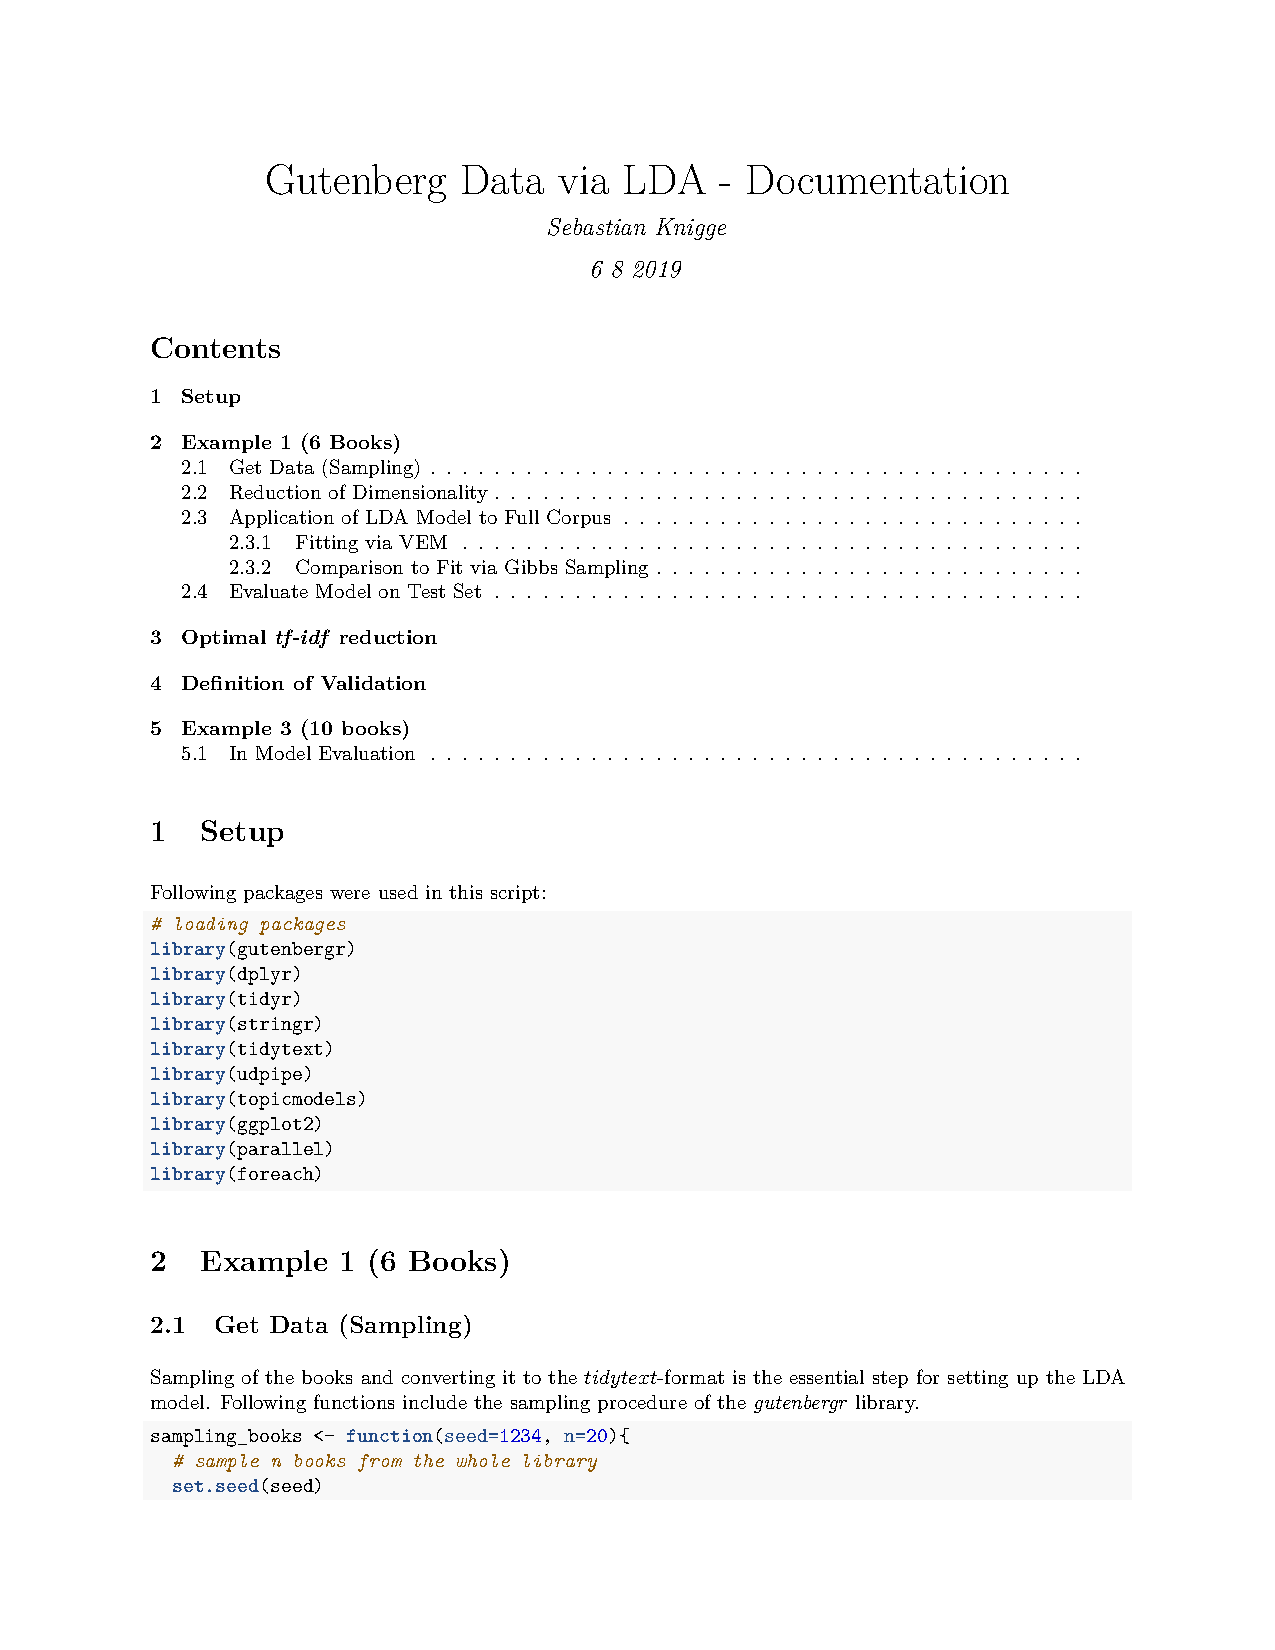
\includepdf[pages=-, pagecommand={}]{LDA_Documentation.pdf}	
\fakesubsection{Documentation of ANN - Gutenberg Data}
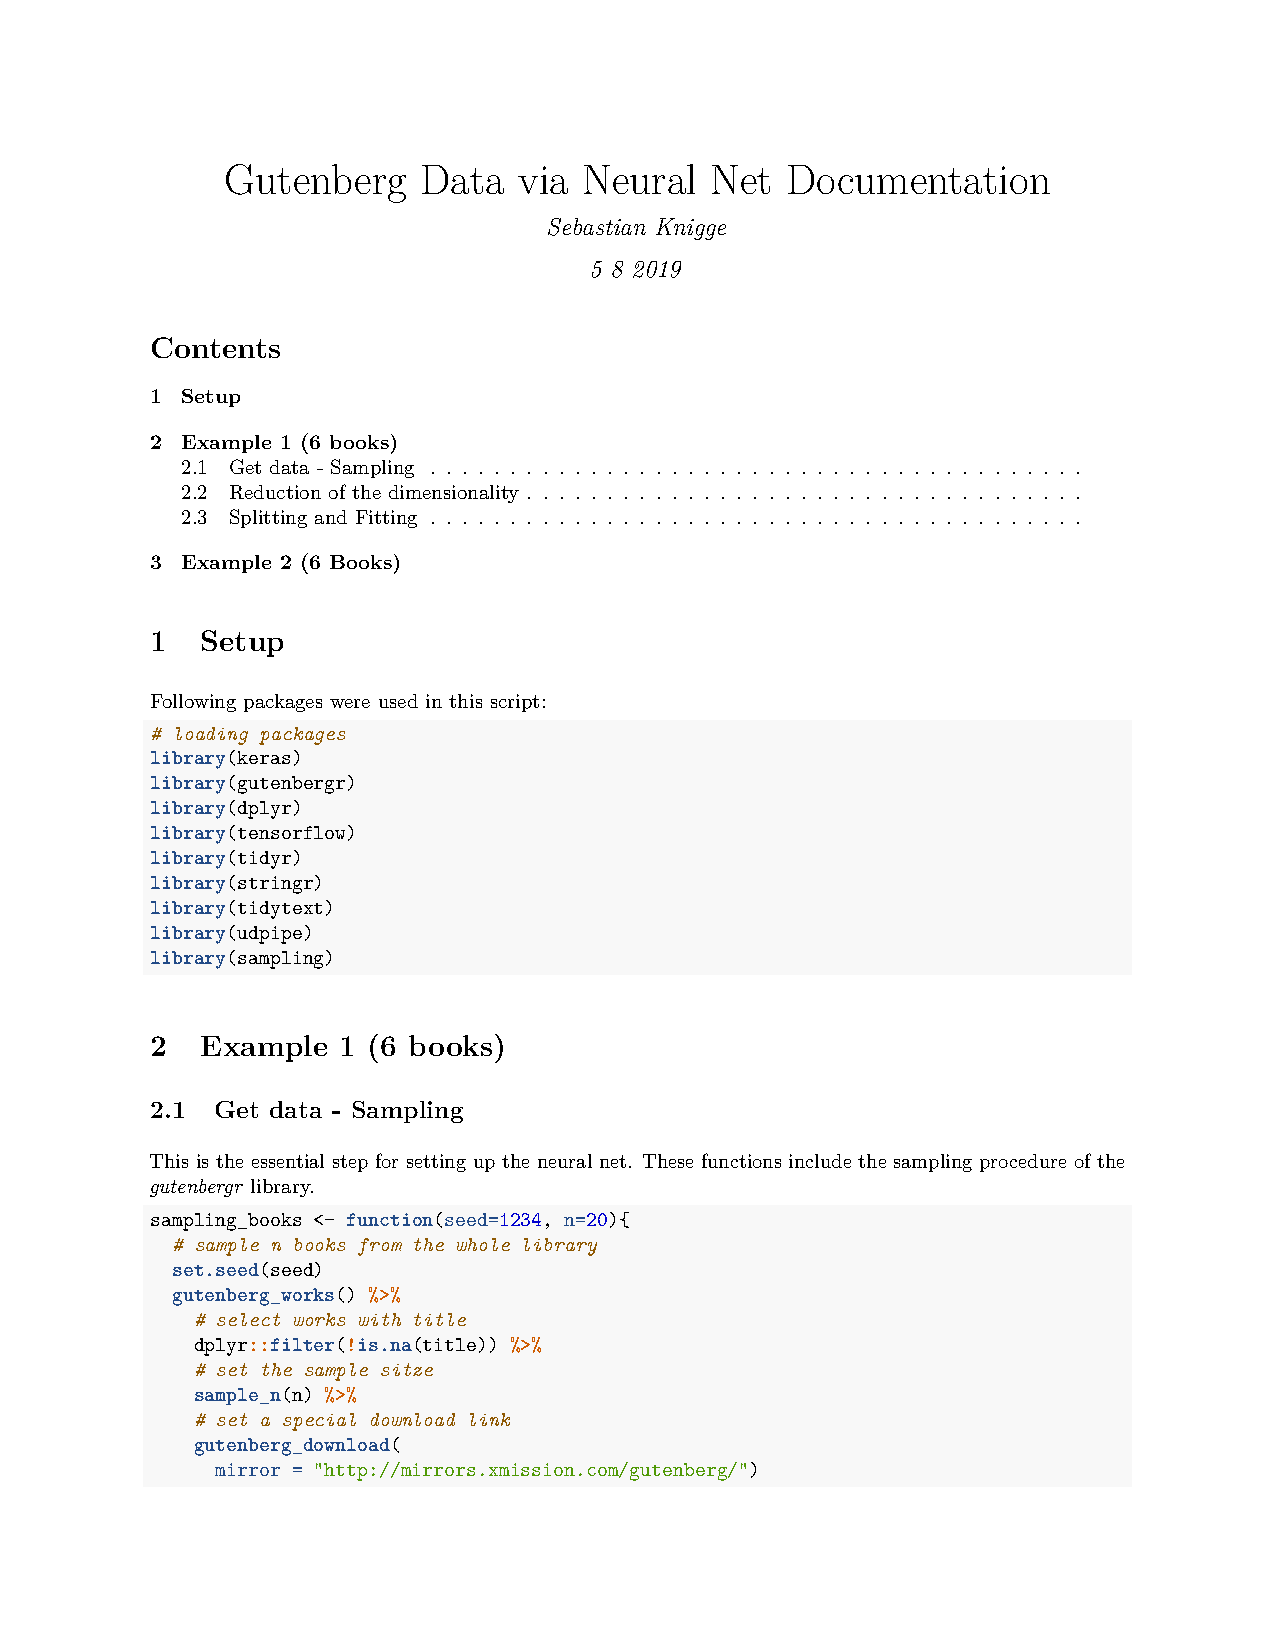
\includepdf[pages=-, pagecommand={}]{NN_Documentation.pdf}




	
\end{document}